\documentclass[12pt]{article}
\usepackage{graphicx} % Required for inserting images
\usepackage[top=1.5cm, left=1.5cm, right=1.5cm, bottom=1.5cm]{geometry}
\usepackage{amsmath}
\usepackage{amsfonts}
\usepackage{amssymb}
\usepackage{amsthm}
\usepackage{hyperref}
\usepackage{tikz}

\title{Friday Question Set}
\author{Eason Shao \and Aidan Wong}
\date{01/05/2024}

\begin{document}

    \maketitle

    \section{Questions}
        \subsection{Question 1}
            This is the equation of a heart:
            \[x^{2}+(y-\sqrt[3]{x^{2}})^{2}=9\]
            
            It represents your love for mathematics.

            An arrow (a metaphor for our test) has been shot through your heart in a particular way: it entered through the point \(A\) on the heart which has the smallest \(x\)-coordinate on the curve, and exited where the heart crosses the point \(B\) which is on the positive \(x\)-axis, as shown in the diagram on the next page.

            \begin{figure}
                \centering
                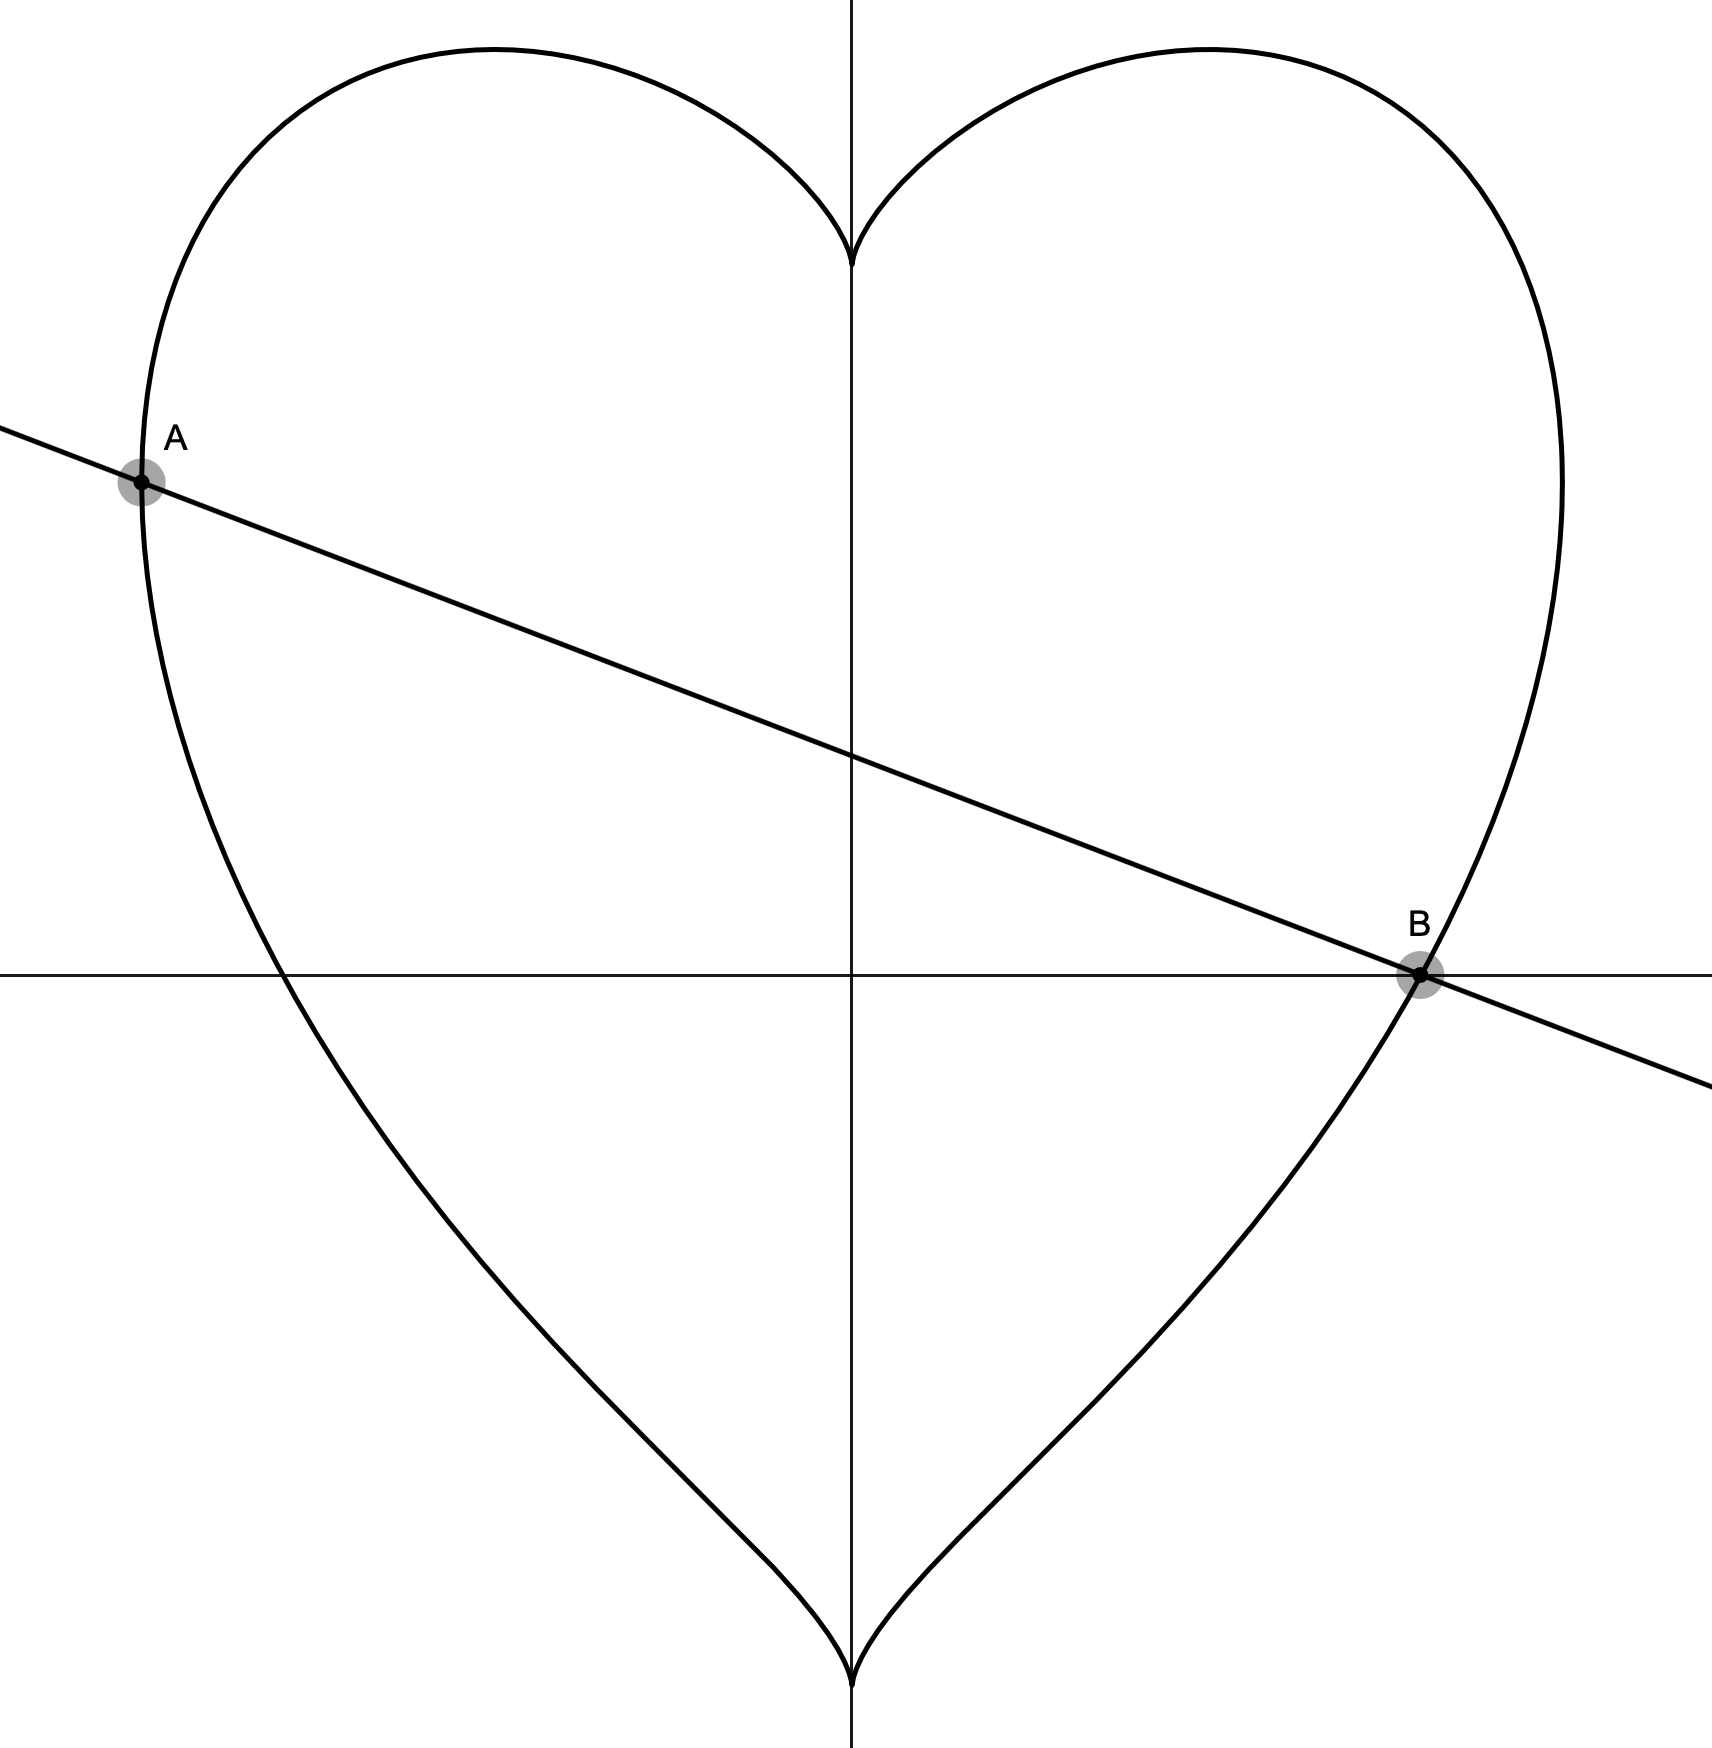
\includegraphics[width = 0.5\textwidth]{Heart.png}
                \caption{Diagram for Question 1}
                \label{fig:Q1Dia}
            \end{figure}
            
            Using implicit differentiation, calculate the distance the arrow has travelled through the heart \(|AB|\).

            \textit{You may assume without proof that point \(A\) has a tangent parallel to the \(y\)-axis}.

            \hfill\textbf{Total for Question [5]}
    
        \subsection{Question 2}
            This question aims to give a well-known upper bound for $\pi$.
    
            \begin{enumerate}
                \item Using the indefinite integral, find the exact value of
                    \[
                    \int_0^1 \left(x^6 - 4x^5 + 5x^4 - 4x^2 + 4\right) \mathrm{d}x. \tag*{\textbf{[2]}}
                    \]
                    
                \item By expressing as a single fraction, without using differentiation, show that
                    \[
                    x^6 - 4x^5 + 5x^4 - 4x^2 + 4 - \frac{4}{1+x^2} \geq 0. \tag*{\textbf{[2]}}
                    \]
                    
                \item Conclude carefully, using an integral, that \(\pi < \frac{22}{7}\).
                    \hfill\textbf{[2]}
            \end{enumerate}
            
            \hfill\textbf{Total for Question [6]}
    
        \subsection{Question 3}
            \begin{enumerate}
                \item By factorising and using a suitable substitution, find
                \[
                    \int (x + \sin x + x \cos x + \sin x \cos x )\mathrm{d}x.
                \]
                \hfill\textbf{Total for Section [2]}

                \item Using suitable trigonometric identities, find
                \[
                    \int (\sin^2 x + \cos^2 x + \tan^2 x + \cot^2 x + \sec^2 x + \csc^2 x) \mathrm{d}x.
                \]
                \hfill\textbf{Total for Section [3]}
            \end{enumerate}
            
            \hfill\textbf{Total for Question [5]}
            
        \subsection{Question 4}
            This question aims to offer a nice insight into optic properties of ellipses.

            We define an \textbf{ellipse} as follows, for \(a > b > 0\):
            \[
            \Gamma: \frac{x^2}{a^2} + \frac{y^2}{b^2} = 1.
            \]

            \begin{figure}
                \centering
                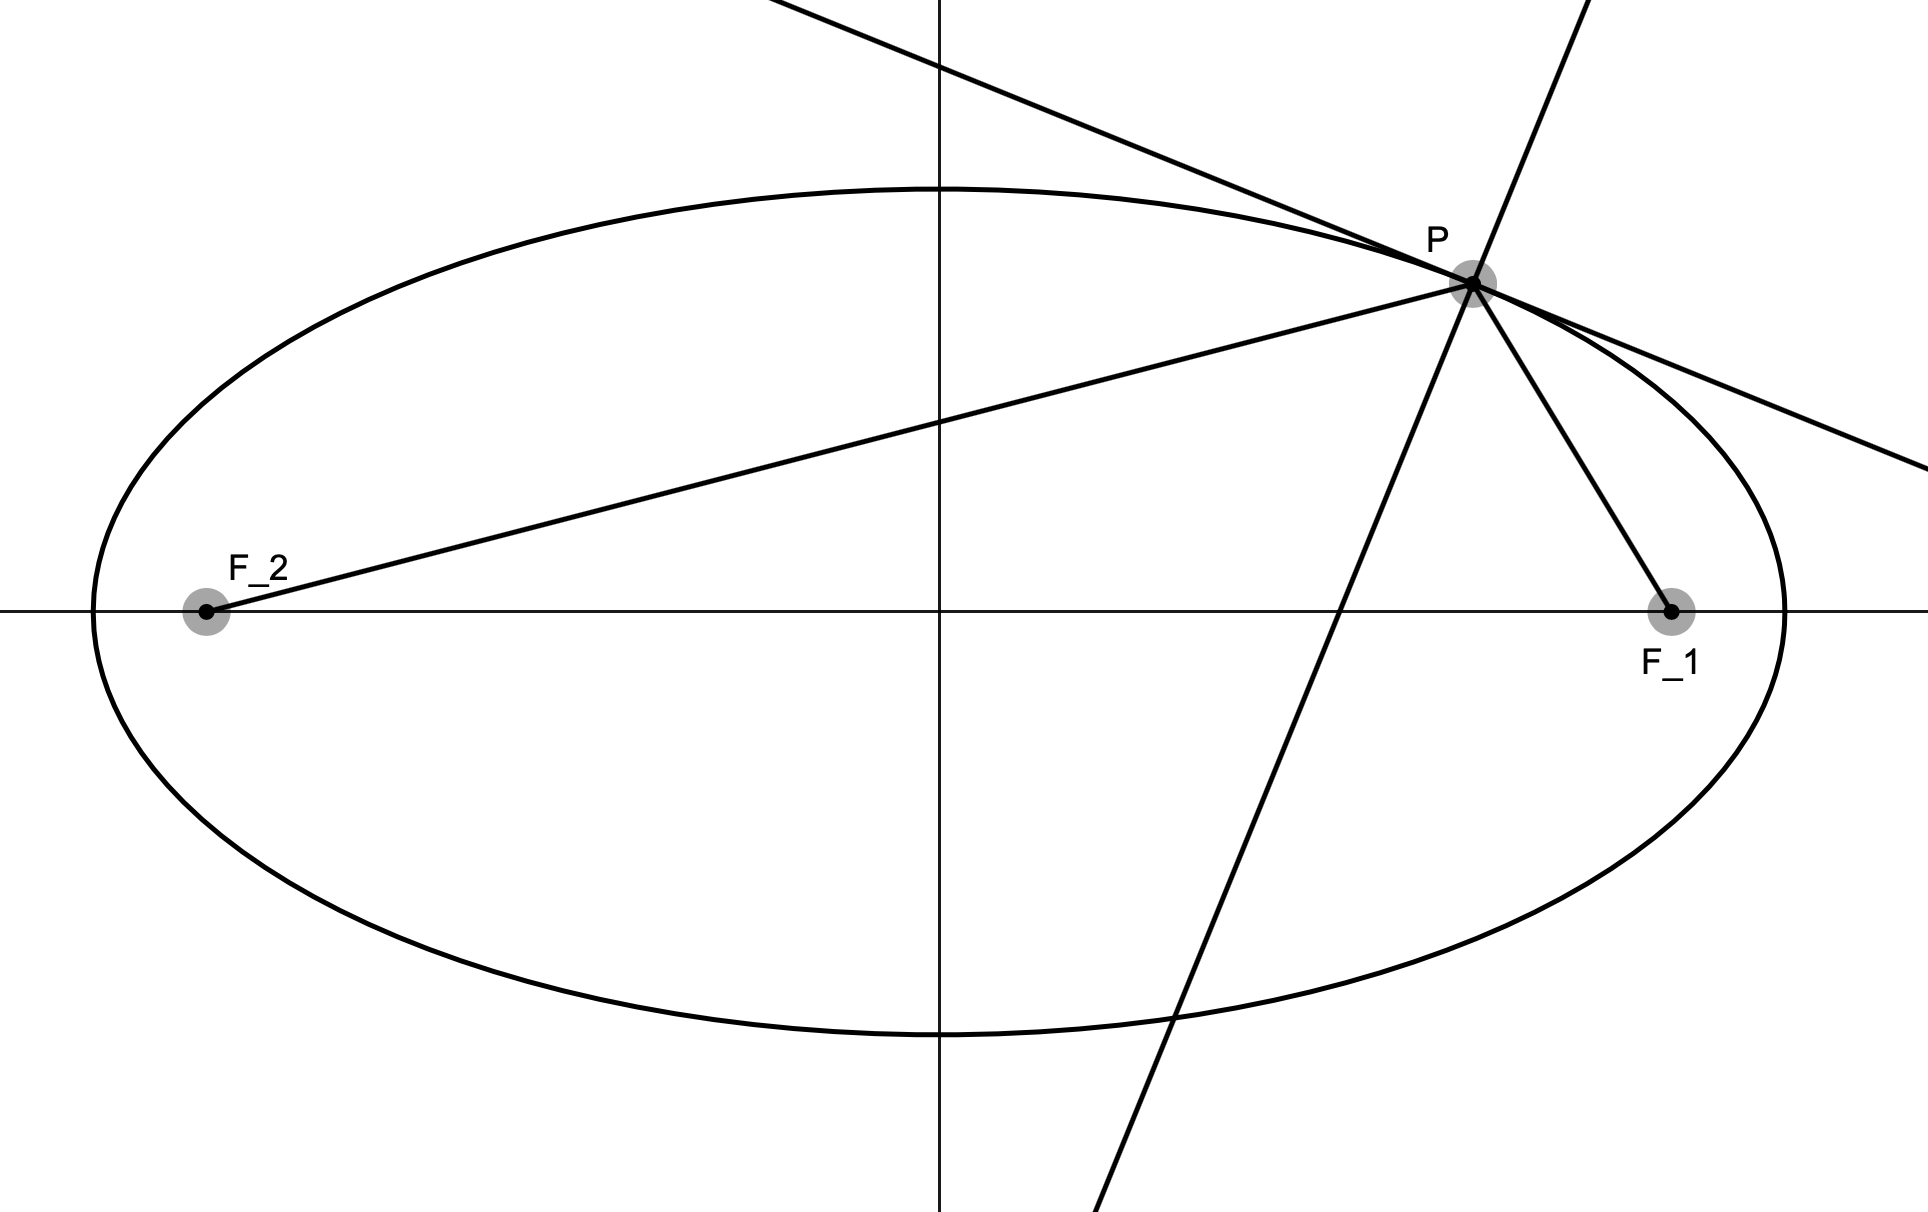
\includegraphics[width = 0.75\textwidth]{Ellipse Diagram.png}
                \caption{Diagram for Question 4}
                \label{fig:Q4Dia}
            \end{figure}

            \begin{enumerate}
                \item Show that there exist two points \(F_1 (c, 0), F_2 (-c, 0)\) where \(c > 0\) satisfying that for any point \(P\) on the ellipse, such that
                \[
                    |PF_1| + |PF_2| = \mathrm{const.}
                \]

                Find \(c\) in terms of \(a\) and \(b\), and also the constant.

                \textit{Such point is in fact unique. You may wish to plug in special values for \(P\) to find the \(c\) and the constant, but you still have to show that such \(c\) gives the same constant for any \(P\).}
                    \hfill\textbf{[4]}

                \item Show, by finding the gradient at a point on the ellipse, that for any light ray from \(F_1\) that is not along the \(x\)-axis, after the first reflection from the ellipse at point \(P\), the reflected light ray passes through the point \(F_2\).

                    \textit{You may use the fact that light reflects along a curve as if there is a mirror along the tangent. In other words, show that the normal at point \(P\) bisects the angle \(\angle F_1 P F_2\).}
                    
                    \hfill\textbf{[5]}
                
            \end{enumerate}
            
            \hfill\textbf{Total for Question [9]}
    
        
        \subsection{Question 5}
            This question is inspired by some scribbles on whiteboards in the Computing/ICT classroom, and aims to offer an insight to the \textbf{Feynman Integration Technique}.

            \textit{You may assume, throughout the question, that all integrals converge.}
    
            \begin{enumerate}
                \item Use an appropriate substitution to show that
                    \[
                    \int_{-\infty}^{+\infty} \sin \exp(x) \mathrm{d}x = \int_{0}^{+\infty} \frac{\sin x}{x} \mathrm{d}x. \tag*{\textbf{[1]}}
                    \]
                    
                \item  We define for \(s \geq 0\) that
                    \[
                    I(s)=\int_0^{+\infty}\frac{\exp(-sx) \sin x \mathrm{d}x}{x}.
                    \]
                    Show that
                    \[
                    \frac{\mathrm{d}}{\mathrm{d}s} I(s) = - \int_0^{+\infty} \exp(-sx) \sin x \mathrm{d}x.
                    \]
                    \textit{You may assume that you can swap the integral and the derivative, i.e.,}
                    \[
                    \frac{\mathrm{d}}{\mathrm{d}s} \int_0^{+\infty} f(s; x) \mathrm{d}x = \int_0^{+\infty} \frac{\mathrm{d}}{\mathrm{d}s} f(s; x) \mathrm{d}x.
                    \]
                    \hfill\textbf{[2]}
            
                \item Using integration by parts twice, or otherwise, show further that
                    \[
                    \frac{\mathrm{d}}{\mathrm{d}s} I(s) = - \frac{1}{1+s^2}. \tag*{\textbf{[3]}}
                    \]
                    
                \item Find the general solution to this differential equation.
                    \hfill\textbf{[1]}
            
                \item  By considering the boundary condition \(\lim_{s \to +\infty} I(s)\), find the particular solution to \(I(s)\).
                
                    \textit{You may assume that you can swap the limit and the integral, i.e., }
                    \[
                    \lim_{s \rightarrow +\infty} \int_0^{+\infty} f(s; x) \mathrm{d}x = \int_0^{+\infty} \lim_{s \rightarrow +\infty} f(s; x) \mathrm{d}x
                    \]
                    \hfill\textbf{[2]}
            
                \item By substituting a suitable value for \(s\) into \(I(s)\), show therefore that
                    \[
                    \int_{-\infty}^{+\infty} \sin \exp(x)  \mathrm{d} x = \frac{\pi}{2}. \tag*{\textbf{[1]}}
                    \]
            \end{enumerate}
            
            \hfill\textbf{Total for Question [10]}\\
        
        \hfill\textbf{Total for Paper [35]}

    \newpage
    
    
    
    
    \section{Solutions}
    
        \subsection{Question 1}
            \textit{Proposed by AW. Solution by AW.}

            By implicit differentiation, we have
            \begin{align*}
                x^2 + \left(y - \sqrt[3]{x^2}\right)^2 &= 9\\
                x^2 + y^2 - 2yx^{\frac{2}{3}} + x^{\frac{4}{3}} &= 9\\
                2x \frac{\mathrm{d}x}{\mathrm{d}y} + 2y - 2x^{\frac{2}{3}} - \frac{4}{3}yx^{-\frac{1}{3}} \frac{\mathrm{d}x}{\mathrm{d}y} + \frac{4}{3} x^\frac{1}{3} \frac{\mathrm{d}x}{\mathrm{d}y} &= 0\\
                \frac{\mathrm{d}x}{\mathrm{d}y} \left(2x - \frac{4}{3} y x^{-\frac{1}{3}} + \frac{4}{3}x\right) &= 2x^{\frac{2}{3}} - 2y\\
                \frac{\mathrm{d}x}{\mathrm{d}y} &= \frac{3x^{\frac{2}{3}} - 3y}{3x - 2y x^{-\frac{1}{3}} + 2x}.
            \end{align*}
            \[\tag*{Correct Implicit Differentiation \textbf{[1]}}\]

            Since \(A\) has vertical tangent, we will know that
            \[
                \frac{\mathrm{d}x}{\mathrm{d}y} = 0 \implies y = x^{\frac{2}{3}}
            \]
            \[\tag*{Attempt to Substitute 0 or infinity \textbf{[1]}}\]

            Substituting back to the original equation gives us
            \[
                x^2 + x^{\frac{4}{3}} - 2x^{\frac{4}{3}} + x^{\frac{4}{3}} = 9 \implies x = \pm 3.
            \]

            By the diagram we will know that \(x = -3\) for \(A\).
            
            Therefore \(A(-3, 2.08)\).\hfill{Correct coordinate for \(A\) \textbf{[1]}}

            By substituting \(y = 0\), we will have that
            \[
                x^2 + x^{\frac{4}{3}} = 9,
            \]
            which gives that \(x = 2.40\) for \(B\). \hfill{Correct coordinate for \(B\) \textbf{[1]}}

            Therefore, the distance will be
            \[
                |AB| = \sqrt{(0 - 2.08)^2 + (2.40 - (-3))^2} = 5.79. \tag*{Correct result for distance \textbf{[1]}}
            \]
            
            \hfill\textbf{Total for Question [5]}
    
        \subsection{Question 2}
            \textit{Adapted from 1968 Putnam by ES.}
            \begin{enumerate}
                \item
                    \begin{align*}
                        \int_0^1 \left(x^6 - 4x^5 + 5x^4 - 4x^2 + 4\right) \mathrm{d}x &= \left[\frac{x^7}{7} - \frac{2x^6}{3} + x^5 - \frac{4x^3}{3} + 4x\right]_{x=0}^{1}
                        \tag*{Correct Primitive Function \textbf{[1]}}\\
                        &= \frac{1}{7} - \frac{2}{3} + 1 - \frac{4}{3} + 4\\
                        &= \frac{22}{7}.
                        \tag*{Convincing Solution \textbf{[1]}}
                    \end{align*}

                    \hfill\textbf{Total for Section [2]}
                    
                \item 
                    \begin{align*}
                        x^6 - 4x^5 + 5x^4 - 4x^2 + 4 - \frac{4}{1+x^2} &= \frac{(1+x^2)(x^6 - 4x^5 + 5x^4 - 4x^2 + 4) - 4}{1+x^2}\\
                        &= \frac{x^8 - 4x^7 + 6x^6 - 4x^5 + x^4}{1+x^2}\\
                        &= \frac{x^4 (1-x)^4}{1+x^2}. \tag*{Correct Manipulation \textbf{[1]}}
                    \end{align*}

                    Notice that for \(x \in \mathbb{R}\), we have \(x^4 \geq 0, (1-x)^4 \geq 0, 1 + x^2 > 0\), hence it is non-negative.
                    
                    \hfill{Convincing Argument \textbf{[1]}}
                    
                    \hfill\textbf{Total for Section [2]}
                    
                \item Since evaluating the integral
                    \[
                        \int_0^1 \frac{x^4 (1-x)^4}{1+x^2} \mathrm{d}x = \frac{22}{7} - \pi,  
                        \tag*{Correct Integral \textbf{[1]}}
                    \]
                    and that the integrand is non-negative and \underline{zero only at finitely many points (\(x = 0, x = 1\))}, we will know that the integral must be positive, and hence rearranging gives us \(\pi < \frac{22}{7}\).
                    
                    \hfill{Must Mention Underlined, Convincing Argument \textbf{[1]}}
                    
                    \hfill\textbf{Total for Section [2]}
            \end{enumerate}
            
            \hfill\textbf{Total for Question [6]}
    
        \subsection{Question 3}
            \textit{Adapted from MIT Integration Bee qualifiers 2023.}
            \begin{enumerate}
                \item We notice that
                \begin{align*}
                    \int (x + \sin x + x \cos x + \sin x \cos x) \mathrm{d}x &= \int (x + \sin x)(1 + \cos x) \mathrm{d}x \tag*{Attempt to factorise \textbf{[1]}}\\
                    &= \int (x + \sin x) \mathrm{d} (x + \sin x)\\
                    &= \frac{(x + \sin x)^2}{2} + C \tag*{Correct result \textbf{[1]}}.
                \end{align*}
                \hfill\textbf{Total for Section [2]}

                \item We notice that
                \begin{align*}
                    \text{Original Integral} &= \int (\sin^2 x + \cos^2 x + \tan^2 x + \cot^2 x + \sec^2 x + \csc^2 x) \mathrm{d}x\\
                    &= \int (1 + \sec^2 x - 1 + \csc^2 x - 1 + \sec^2 x + \csc^2 x)\mathrm{d}x \tag*{Attempt to use any  of three trigonometric identity \textbf{[1]}}\\
                    & \tag*{Correctly using all three trigonometric identities \textbf{[1]}}\\
                    &= \int (-1 + 2\sec^2 x + 2\csc^2 x) \mathrm{d}x\\
                    &= -x + 2\tan x - 2\cot x + C. \tag*{Correct result \textbf{[1]}}
                \end{align*}
                
                \hfill\textbf{Total for Section [3]}
            \end{enumerate}
            \hfill\textbf{Total for Question [5]}
    
        \subsection{Question 4}
            \textit{Proposed by AW and ES. Solution by ES.}
            \begin{enumerate}
                \item 
                    Set the coordinates of the point \(P\) as \(P(x, y)\). 

                    We notice that
                    \[
                        d(x, y) = |PF_1| + |PF_2| = \sqrt{(x - c)^2 + y^2} + \sqrt{(x + c)^2 + y^2}.
                    \]

                    If \(d(x, y)\) is a constant for all \(P(x, y)\), then it must satisfy for \(P(a, 0)\) and \(P(0, b)\)
                    \[
                        d(a, 0) = d(0, b).
                    \]

                    Therefore, by plugging in values, we have
                    \[
                        2\sqrt{b^2 + c^2} = d(a, 0) = d(0, b) = 2a,
                    \]
                    which gives us 
                    \[
                        c = \sqrt{a^2 - b^2}, \tag*{Correct Result \textbf{[1]}}
                    \]
                    and
                    \[
                        d(x, y) = 2a. \tag*{Correct Result \textbf{[1]}}
                    \]

                    Notice that
                    \[
                        \frac{x^2}{a^2} + \frac{y^2}{b^2} = 1 \iff y^2 = b^2 - \frac{x^2 b^2}{a^2}. \tag*{Any Utilize of Definition \textbf{[1]}}
                    \]

                    We still have to show that \(P(x, y) \equiv 2a\) for \(c^2 = a^2 - b^2\) on the curve.
                    \begin{align*}
                        d(x, y)^2 &= (x+c)^2 + y^2 + (x-c)^2 + y^2 + 2 \sqrt{\left[(x-c)^2 +y^2\right] \left[(x+c)^2 + y^2\right]}\\
                        &= 2 \left[x^2 + y^2 + a^2 - b^2 + \sqrt{\left(x^2 + y^2 + a^2 - b^2\right)^2 - 4x^2c^2}\right]\\
                        &= 2 \left[x^2 + a^2 - \frac{x^2 + b^2}{a^2} + \sqrt{\left(x^2 + a^2 - \frac{x^2 b^2}{a^2}\right)^2 - 4x^2(a^2 - b^2)}\right]\\
                        &= 2 \left[x^2 + a^2 - \frac{x^2 + b^2}{a^2} + \sqrt{\left(x^2 - a^2 - \frac{x^2 b^2}{a^2}\right)^2}\right]\\
                        &= 2 \left[x^2 + a^2 - \frac{x^2 + b^2}{a^2} - \left(x^2 - a^2 - \frac{x^2 b^2}{a^2}\right) \right]\\
                        &= 4a^2
                    \end{align*}
                    as desired.
                    \hfill{Convincing Proof \textbf{[1]}}
                    
                    \hfill\textbf{Total for Section [4]}

                \item
                    Leg the normal to \(\Gamma\) at \(P\) meet the \(x\)-axis at \(Q\).

                    By implicit differentiation, it is not difficult to see that
                    \[
                        \frac{\mathrm{d}y}{\mathrm{d}x} = - \frac{b^2 x}{a^2 y},
                    \]
                    and therefore, the gradient of the normal will be
                    \[
                        \frac{\mathrm{d}x}{\mathrm{d}y} = \frac{a^2 y}{b^2 x}. \tag*{Correct Gradient \textbf{[1]}}
                    \]

                    This means that
                    \[
                        \tan \angle PQF_1 = \frac{a^2 y}{b^2 x}, \tan \angle PQF_2 = - \frac{a^2 y}{b^2 x}.
                    \]

                    Also, by gradient of a line, we have
                    \[\tan \angle PF_2 Q = \frac{a}{c + x}, \tan \angle PF_1 Q = \frac{1}{c - x} \tag*{Correct Gradients \textbf{[1]}}\]

                    By using the fact that
                    \[
                    \tan (\pi - A - B) = - \tan(A + B) = -\frac{\tan A + \tan B}{1 - \tan A \tan B}, \tag*{Attempt of Use of Formula \textbf{[1]}}
                    \]
                    we will find that
                    \begin{align*}
                        \tan \angle F_2 PQ &= - \frac{\frac{y}{c + x} - \frac{a^2 y}{b^2 x}}{1 + \frac{a^2 y^2}{b^2 x (c+x)}}\\
                        &= \frac{a^2 cy + a^2 xy - b^2 xy}{b^2 cx + b^2 x^2 + a^2 y^2}\\
                        &= \frac{a^2 cy + c^2 xy}{b^2 cx + a^2 b^2} \tag*{Attempt to Substitute Values \textbf{[1]}}\\
                        &= \frac{cy (a^2 + cx)}{b^2 (a^2 + cx)}\\
                        &= \frac{cy}{b^2} \tag*{Tangent Value Correct \textbf{[1]}},
                    \end{align*}
                    and
                    \begin{align*}
                        \tan \angle F_1 PQ &= - \frac{\frac{y}{c - x} - \frac{a^2 y}{b^2 x}}{1 - \frac{a^2 y^2}{b^2 x (c+x)}}\\
                        &= \frac{a^2 xy - b^2 xy - a^2 cy}{b^2 cx - b^2 x^2 - a^2 y^2}\\
                        &= \frac{c^2 xy - a^2 cy}{b^2 cx - a^2 b^2}\\
                        &= \frac{cy (cx - a^2)}{b^2 (cx - a^2)}\\
                        &= \frac{cy}{b^2}.
                    \end{align*}
                    
                     Therefore\(\angle F_2 PQ = \angle F_1 PQ\) as desired.
                    \hfill{Convincing and Complete Proof \textbf{[1]}}
                    
                    \hfill\textbf{Total for Section [5]}
            \end{enumerate}
            
            \hfill\textbf{Total for Question [9]}
        
        \subsection{Question 5}
            \textit{Inspired by scribbles on the whiteboard in SPS Room 217. Solution adapted from \href{https://math.stackexchange.com/questions/2322547/improper-integral-of-sinx-x-from-zero-to-infinity}{Maths Stack Exchange \#2322547} with credits to R. Feynman. Refined by Eason Shao.}
            \begin{enumerate}
                \item By substituting \(u = \exp(x)\), we will have \(u \to 0\) as \(x \to -\infty\) and \(u \to +\infty\) as \(x \to +\infty\), and \(\frac{\mathrm{d}u}{\mathrm{d}x} = u\). Therefore
                    \begin{align*}
                        \int_{-\infty}^{+\infty} \sin \exp(x) \mathrm{d}x &= \int_0^{+\infty} \frac{\sin u}{u} \mathrm{d}u\\
                        &= \int_0^{+\infty} \frac{\sin x}{x} \mathrm{d}x. \tag*{Convincing Explanation \textbf{[1]}}
                    \end{align*}
                
                    \hfill\textbf{Total for Section [1]}
                    
                \item  
                    \begin{align*}
                        \frac{\mathrm{d}}{\mathrm{d}s} I(s) &= \frac{\mathrm{d}}{\mathrm{d}s} \int_0^{+\infty}\frac{\exp(-sx) \sin x \mathrm{d}x}{x}\\
                        &= \int_0^{+\infty} \frac{\mathrm{d}}{\mathrm{d}s}  \frac{\exp(-sx)\sin x \mathrm{d}x}{x} \tag*{Attempt to Swap \textbf{[1]}}\\
                        &= \int_0^{+\infty} -x \frac{\exp(-sx)\sin x \mathrm{d}x}{x}\\
                        &= - \int_0^{+\infty} \exp(-sx)\sin x \mathrm{d}x. \tag*{Convincing Proof \textbf{[1]}}
                    \end{align*}


                    \hfill\textbf{Total for Section [2]}
            
                \item 
                    Note that
                    \begin{align*}
                        \int \exp(-sx) \sin x \mathrm{d}x &= \int \sin x \mathrm{d} \left(- \frac{1}{s} \exp(-sx)\right)\\
                        &= -\frac{\exp(-sx) \sin x}{s} + \frac{1}{s} \int \exp(-sx) \mathrm{d} \sin x\\
                        &= -\frac{\exp(-sx) \sin x}{s} + \frac{1}{s} \int \exp(-sx) \cos x \mathrm{d}x \tag*{Attempt of Integration by Parts \textbf{[1]}}\\
                        &= -\frac{\exp(-sx) \sin x}{s} + \frac{1}{s} \int \cos x \mathrm{d}\left(- \frac{1}{s} \exp(-sx)\right)\\
                        &= - \frac{\exp(-sx) \sin x}{s} - \frac{1}{s^2} \exp(-sx) \cos x + \frac{1}{s^2} \int \exp(-sx) \mathrm{d} \cos x\\
                        &= - \frac{\exp(-sx) \sin x}{s} - \frac{1}{s^2} \exp(-sx) \cos x - \frac{1}{s^2} \int \exp(-sx) \sin x\mathrm{d} x.\\
                    \end{align*}

                    Therefore,
                    \[
                        \left(1 + \frac{1}{s^2}\right) \int \exp(-sx) \sin x = - \exp(-sx) \frac{s\sin x + \cos x}{s^2}, \tag*{Attempt of Manipulation \textbf{[1]}}
                    \]
                    \[
                        \int \exp(-sx) \sin x = - \exp(-sx) \frac{s\sin x + \cos x}{1 + s^2},
                    \]
                    and hence
                    \begin{align*}
                        \frac{\mathrm{d}}{\mathrm{d}s} I(s) &= -\int_{0}^{+\infty} \exp(-sx) \sin x \mathrm{d}x\\
                        &= \left[\exp(-sx) \frac{s \sin x + \cos x}{1+s^2}\right]_{x = 0}^{+\infty}\\
                        &= \left(0\right) - \left(\frac{1}{1+s^2}\right) \tag*{Evaluating Limits \textbf{[1]}}\\
                        &= - \frac{1}{1+s^2}.
                    \end{align*}
                    
                    \hfill\textbf{Total for Section [3]}
                    
                \item 
                    \[I(s) = - \arctan(s) + C. \tag*{Correct Solution with Constant \textbf{[1]}}\]
                    
                    \hfill\textbf{Total for Section [1]}
            
                \item 
                    \begin{align*}
                        \lim_{s \to +\infty} I(s) &= \lim_{s \to +\infty} \int_{0}^{+\infty} \frac{\exp(-sx) \sin x}{x} \mathrm{d}x\\
                        &= \int_{0}^{+\infty} \lim_{s \to +\infty} \frac{\exp(-sx) \sin x}{x} \mathrm{d}x\\
                        &= \int_{0}^{+\infty} 0 \mathrm{d}x\\
                        &= 0. \tag*{Correct Limit \textbf{[1]}}
                    \end{align*}

                    \[I(+\infty) = - \frac{\pi}{2} + C = 0 \implies I(s) = \frac{\pi}{2} - \arctan s. \tag*{Correct Value for Constant \textbf{[1]}}\]
                    
                    \hfill\textbf{Total for Section [2]}
            
                \item
                    \begin{align*}
                         \int_{-\infty}^{+\infty} \sin \exp(x)  \mathrm{d} x &= \int_{0}^{+\infty} \frac{\sin x}{x} \mathrm{d}x\\
                         &= I(0)\\
                         &= \frac{\pi}{2} - \arctan{0}\\
                         &= \frac{\pi}{2}. \tag*{Correct Result \textbf{[1]}}
                    \end{align*}
                    
                    \hfill\textbf{Total for Section [1]}
            \end{enumerate}

            \textit{Remark.} There are numerous ways to solve this integral, after doing the substitution. Links include: 
            
            \begin{enumerate}
                \item \href{https://math.stackexchange.com/questions/2322547/improper-integral-of-sinx-x-from-zero-to-infinity}{Maths Stack Exchange \#2322547} (this solution's \(I(s)\) is based on this);
                \item \href{https://math.stackexchange.com/questions/192685/are-there-any-ways-to-evaluate-int-infty-0-frac-sin-xxdx-without-using-d}{Maths Stack Exchange \#192685};
                \item \href{https://math.stackexchange.com/questions/5248/evaluating-the-integral-int-0-infty-frac-sin-x-x-mathrm-dx-frac-pi}{Maths Stack Exchange \#5248} which includes other excellent methods such as  Fourier Transform, Laplace Transform, Double Integration, ... and I totally do not understand.
            \end{enumerate}
            
            It is also worth mentioning that G.H. Hardy presented two articles on approximately 12 ways to do this integral, with one of them linked \href{https://people.math.harvard.edu/~ctm/home/text/class/harvard/55b/10/html/home/hardy/sinx/sinx.pdf}{here} and the other one in \textit{Math. Gaz.} 8 (July 1916) pp. 301–303., as mentioned in the 3rd link on Stack Exchange. I believe this solution produced here is probably one of the most elegant ones.
            
            \hfill\textbf{Total for Question [10]}\\

        
        \hfill\textbf{Total for Paper [35]}
    

\end{document}

% Aidan: 1 9 4 1 14
% Eason: 5 1 19 15 14